\bgroup
\setbeamercolor{background canvas}{bg=black}
\begin{frame}[plain]



  %\begin{figure}%[htbp]
    %\centering
  \hspace*{-1.05cm} 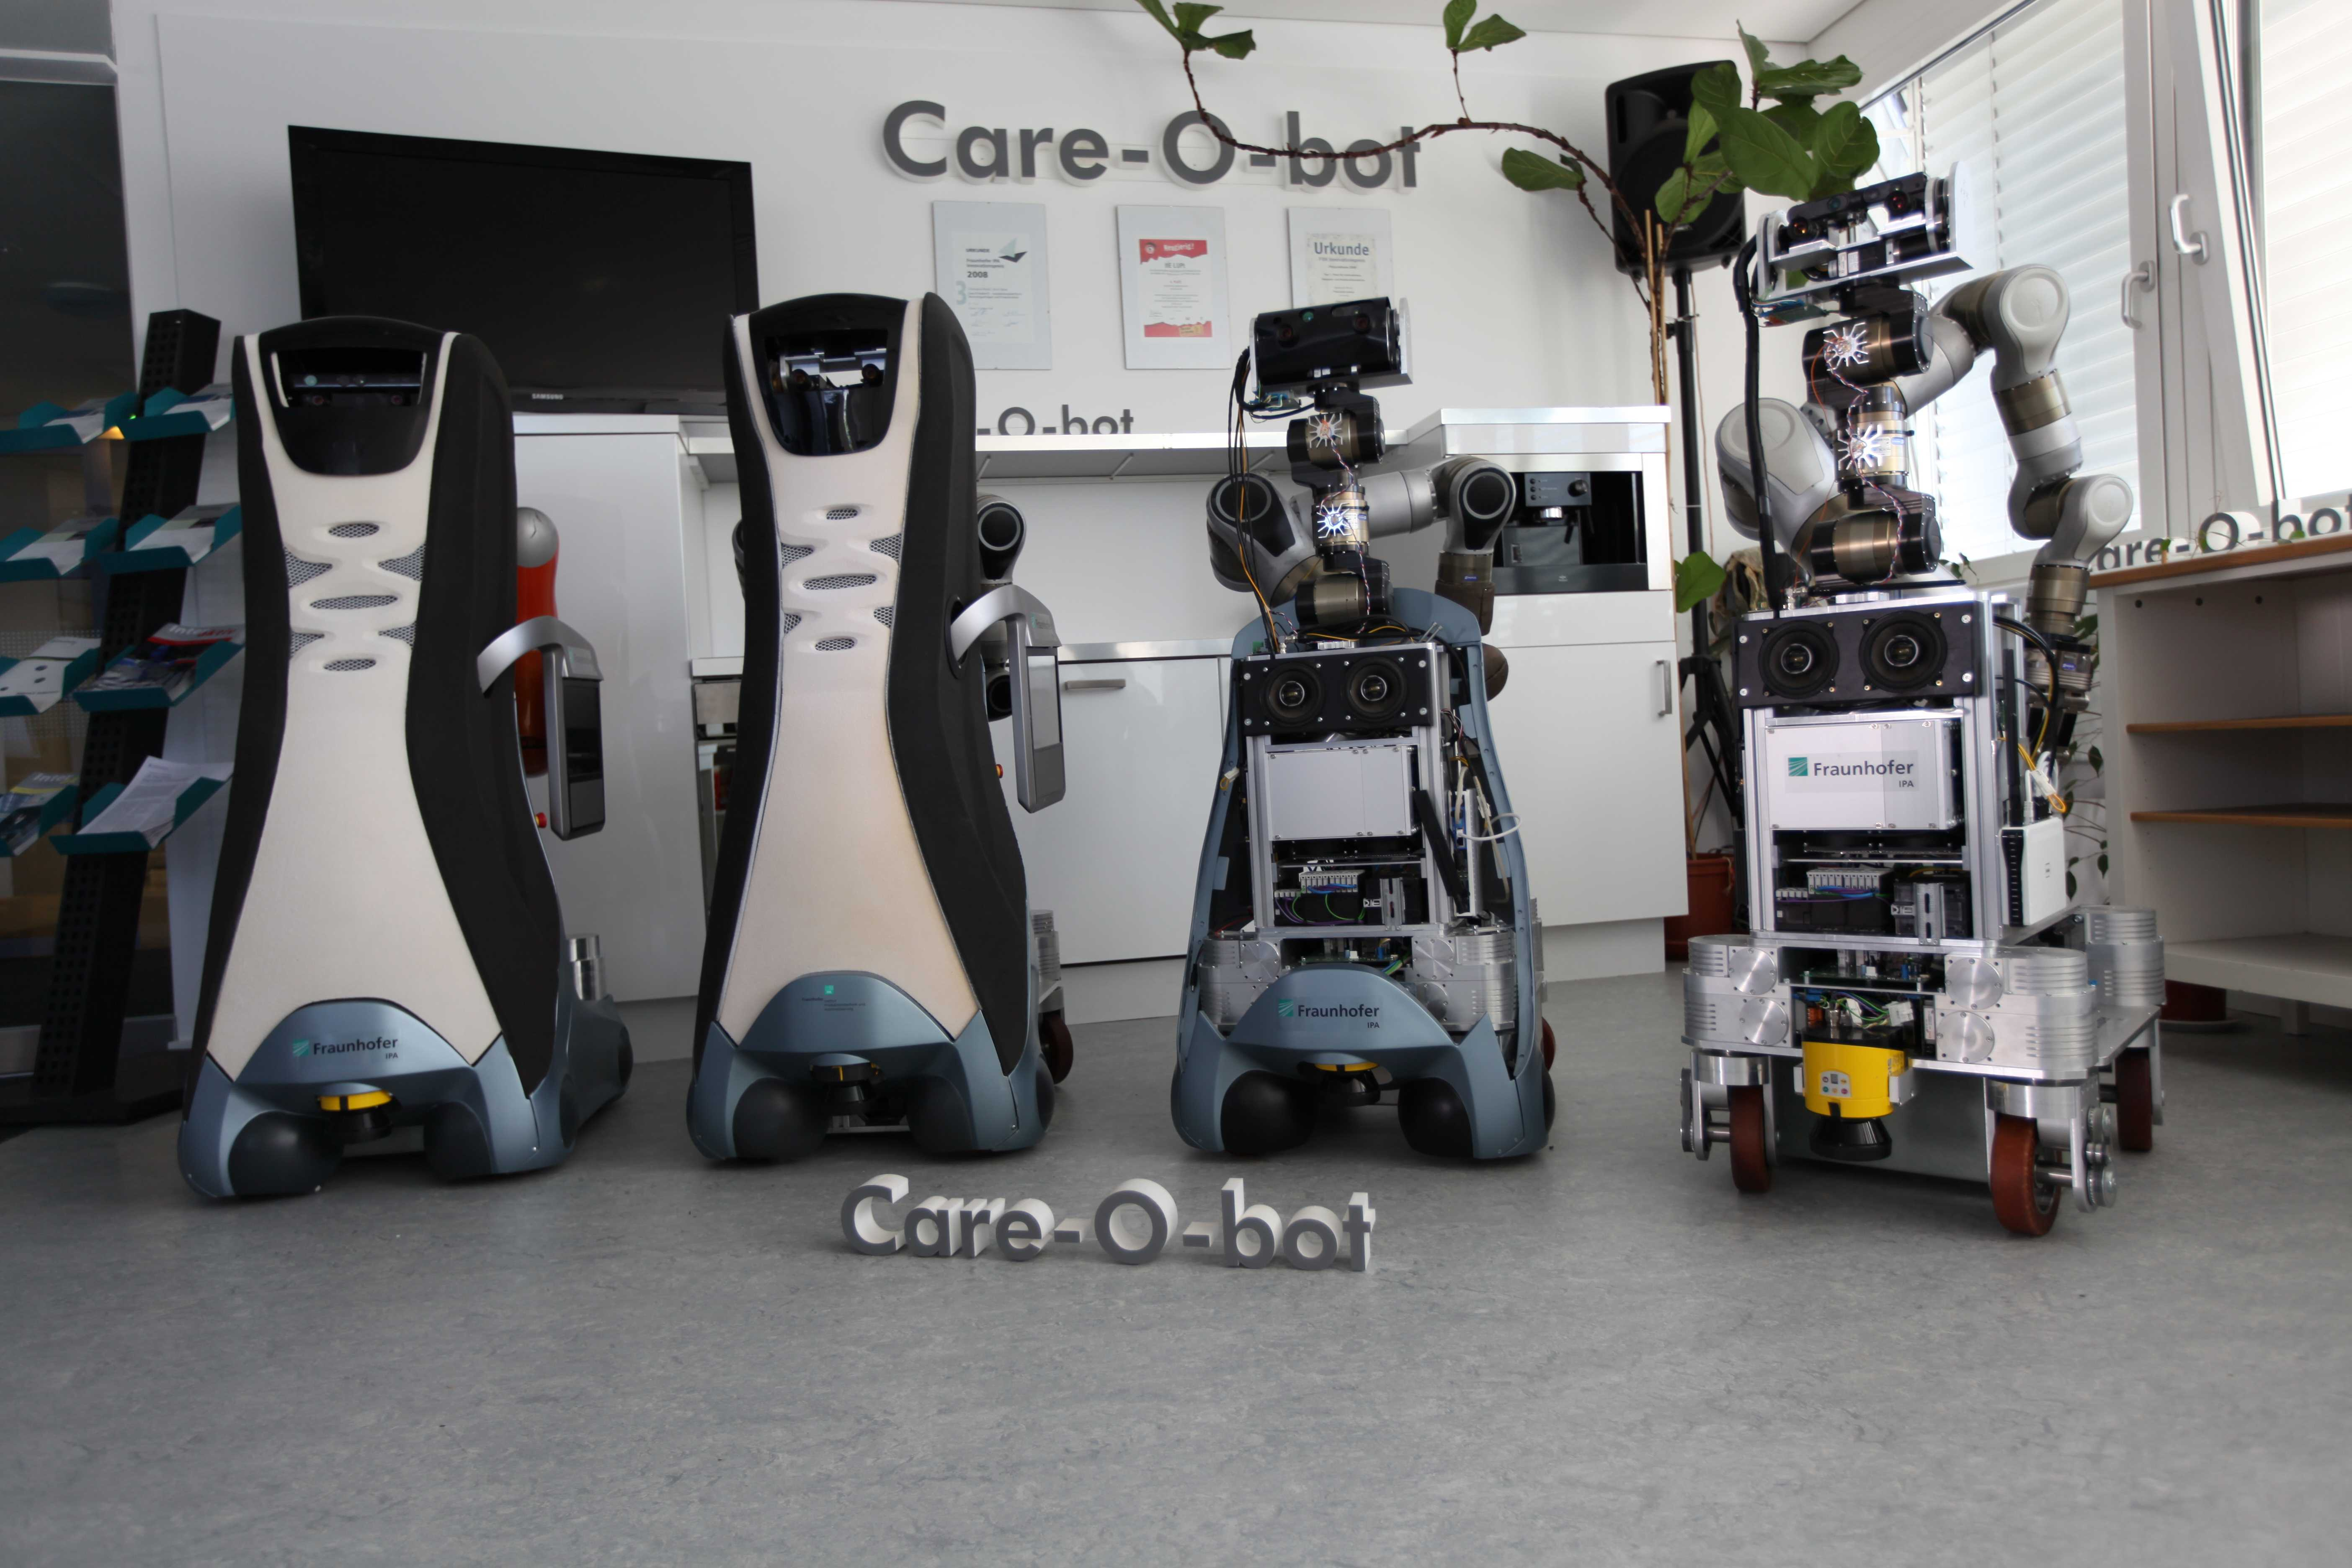
\includegraphics[width=\paperwidth]{images/cobs}
  %\end{figure}
\end{frame}
\egroup


%\begin{frame}

  %\frametitle{Aufbau des \cob}

  %\begin{figure}[htbp]
    %\centering
    %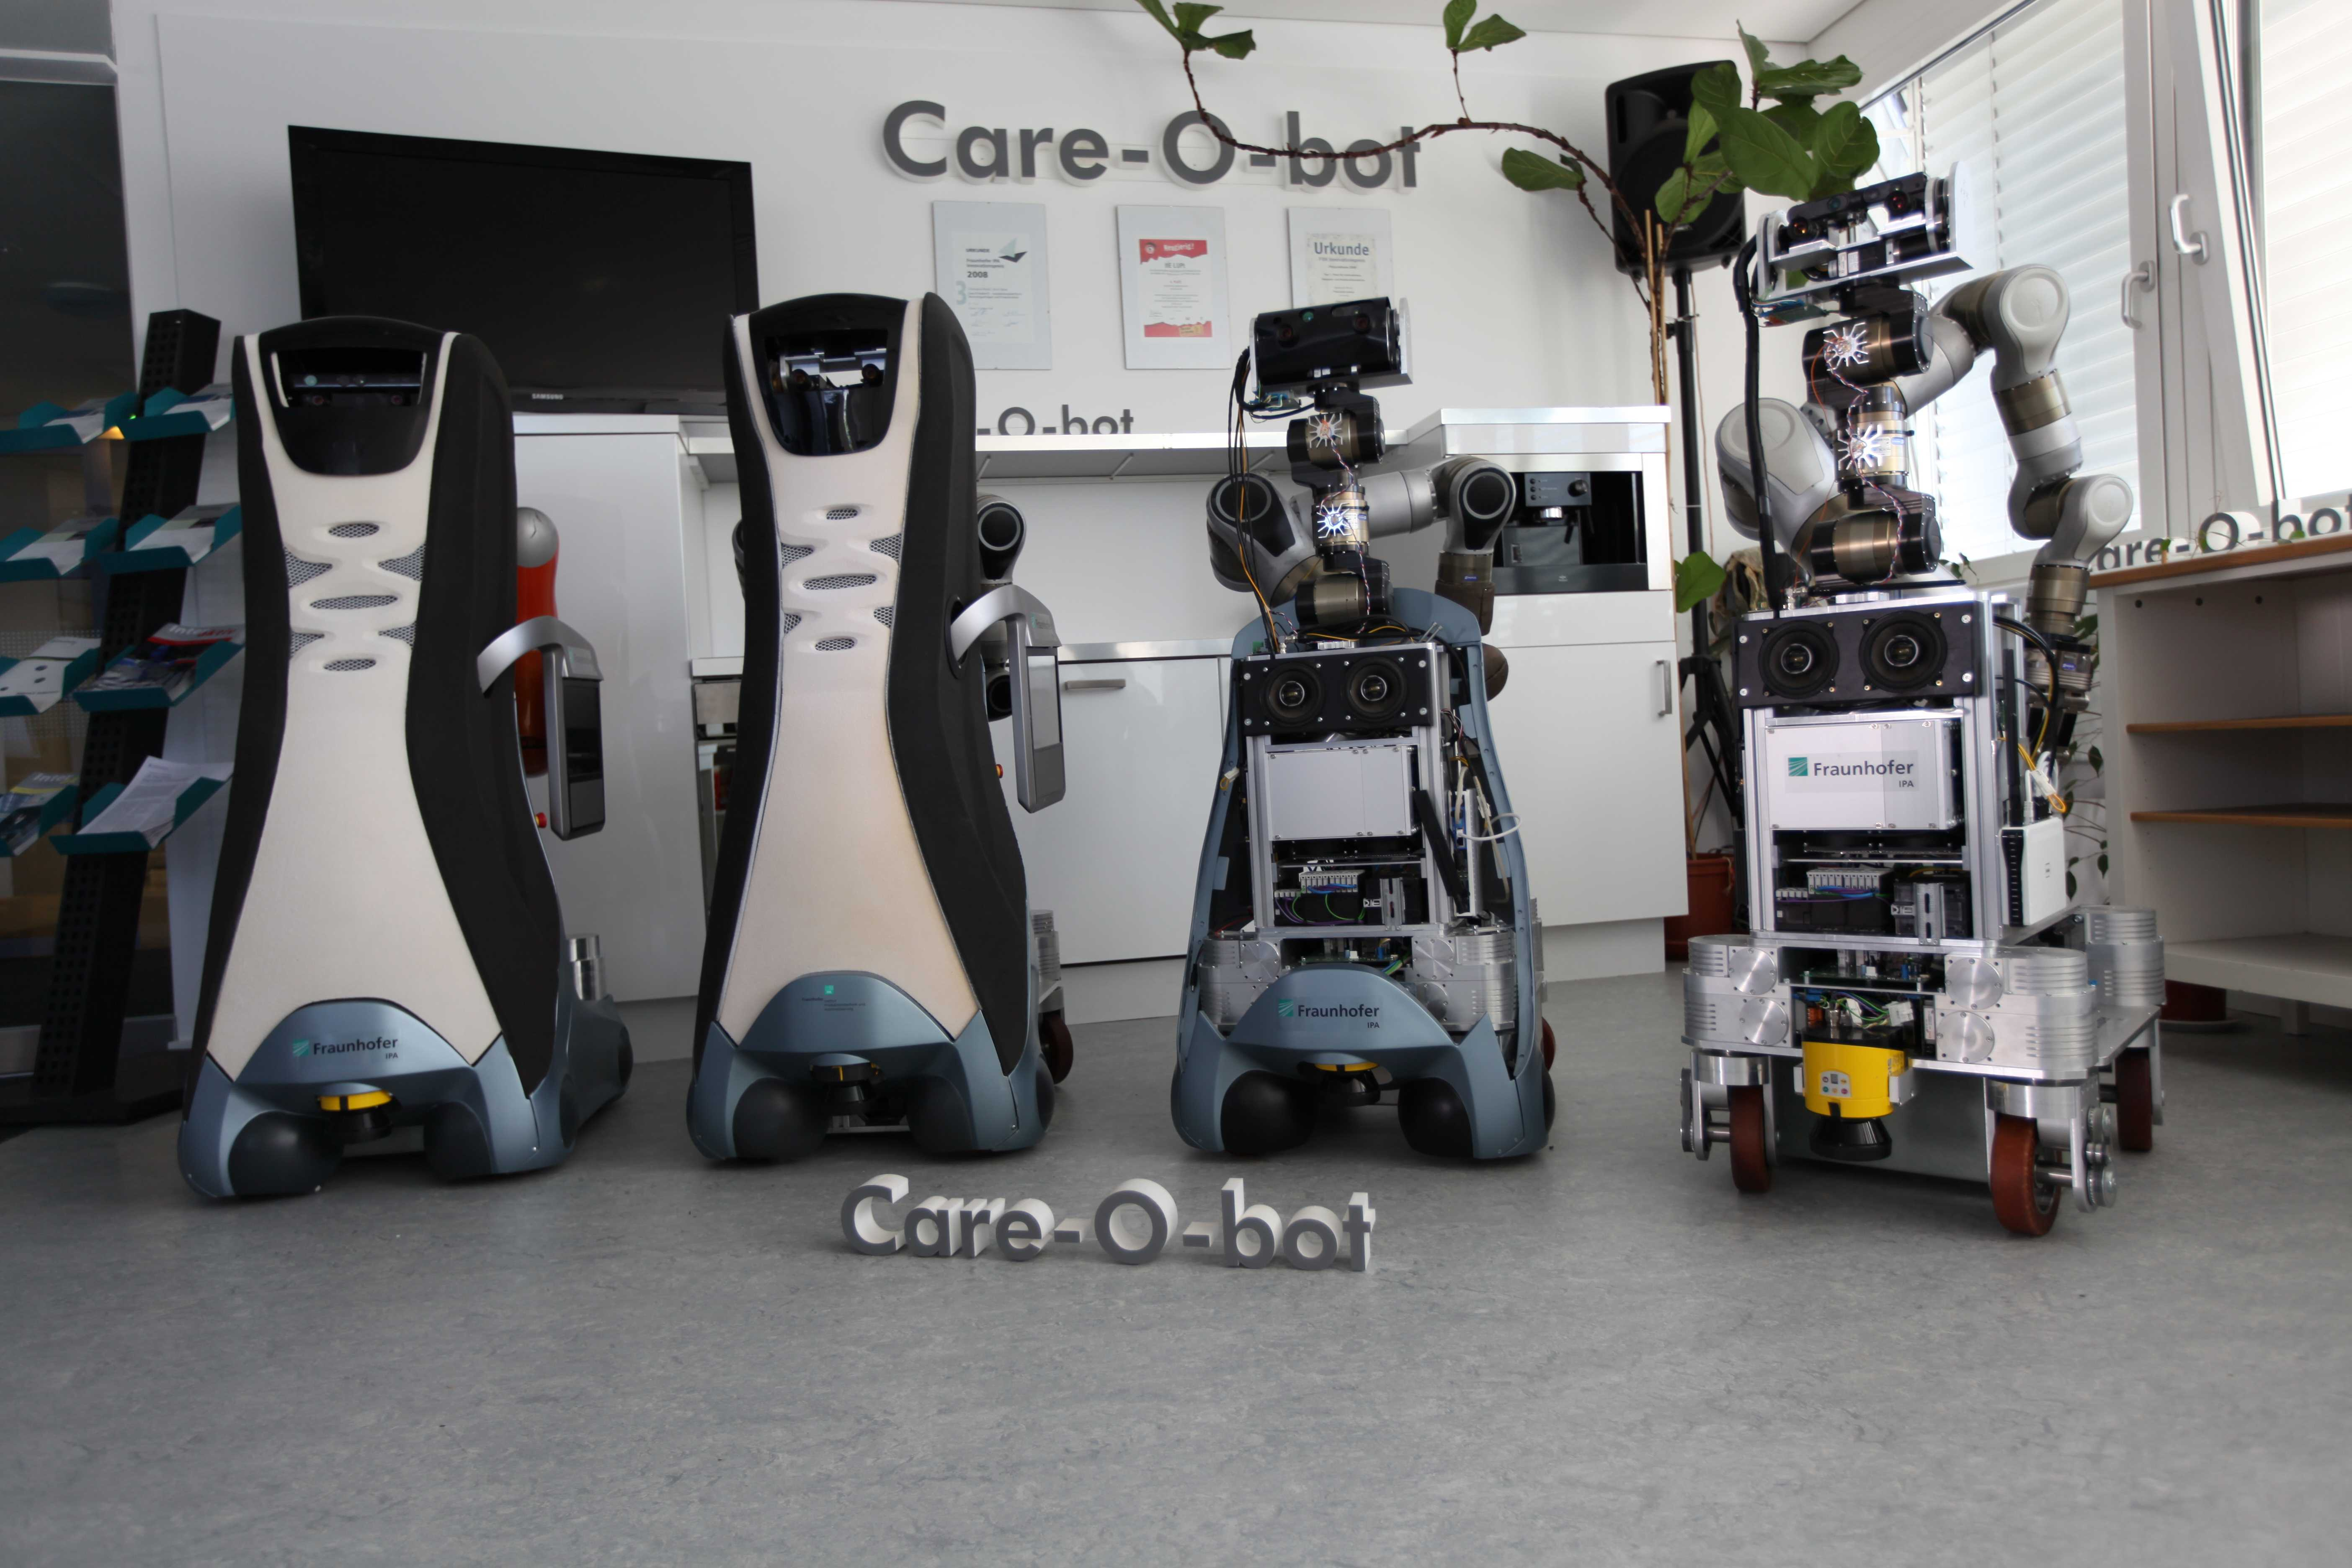
\includegraphics[height=0.65\textheight]{images/cobs}
    %\label{fig:cobs}
  %\end{figure}
%\end{frame}

\placelogofalse
\begin{frame}
  \frametitle{Komponenten des \cob}
\begin{block}
  {Hardware}
\begin{itemize}
    \pause
    \item Kopf mit drei Kameras \pause
    \item Roboterarm mit sieben Freiheitsgraden \pause
    \item Torso auf mobiler Plattform mit mehreren Freiheitsgraden \pause
  \end{itemize}
\end{block}

\pause

\begin{block}{Software}
  \pause
    \begin{itemize}
      \item Ubuntu \pause
      \item Robot-Operating-System \pause
      \item ROS Nodes
    \end{itemize}
  \end{block}
\end{frame}

\placelogotrue
